% ===========================================================================
% Project 8: Explainable Multi-Modal Phishing Detection
% Student: Vaishnavi Purohit (x24260339)
% Institution: National College of Ireland
% Programme: MSc Artificial Intelligence and Machine Learning
% Format: IEEEtran (conference)
% ===========================================================================
\documentclass[conference]{IEEEtran}

\usepackage[utf8]{inputenc}
\usepackage[T1]{fontenc}
\usepackage{amsmath,amssymb,amsthm}
\usepackage{graphicx}
\usepackage{booktabs}
\usepackage{hyperref}
\usepackage{xcolor}
\usepackage{float}
\usepackage{caption}
\usepackage{subcaption}
\usepackage{algorithm}
\usepackage{algpseudocode}
\usepackage{multirow}
\usepackage{enumitem}
\usepackage{array}
\usepackage{tabularx}
\usepackage{boldline}
\usepackage{url}

\hypersetup{
  colorlinks=true,
  linkcolor=blue!70!black,
  citecolor=green!50!black,
  urlcolor=blue!60!black
}

\graphicspath{{../outputs/}}

% ===========================================================================
\title{Explainable Multi-Modal Phishing Detection:\\
       Integrating BERT Transformers with XAI\\
       for Trustworthy Email Security}

\author{
  \IEEEauthorblockN{Vaishnavi Purohit}
  \IEEEauthorblockA{Student ID: x24260339\\
  MSc Artificial Intelligence and Machine Learning\\
  National College of Ireland\\
  Email: x24260339@student.ncirl.ie}
}

\begin{document}

\maketitle

% ---------------------------------------------------------------------------
\begin{abstract}
This work presents an explainable multi-modal phishing detection framework evaluated on 20,847 email samples from seven public sources. Three modalities are extracted per email: text content via fine-tuned DistilBERT, URL structure metadata (15 features), and domain temporal signals (8 features). A late fusion architecture concatenates modality-specific representations before classification. The model achieves F1=0.978, outperforming DistilBERT text-only (F1=0.961) and URL-only (F1=0.934) baselines. Explainability is provided through KernelSHAP, LIME, and DistilBERT attention visualisation, with a novel consistency analysis quantifying inter-method agreement via Kendall's $\tau$ (0.847) and fidelity scores from top-$k$ feature removal. Statistical validation across 10 random seeds with paired $t$-tests confirms all differences are significant.
\end{abstract}

\begin{IEEEkeywords}
Phishing detection, multi-modal learning, late fusion, DistilBERT, explainable AI,
KernelSHAP, LIME, attention visualisation, email security, deep learning
\end{IEEEkeywords}

% ===========================================================================
\section{Introduction}
\label{sec:introduction}

Phishing remains the most prevalent initial access vector in cyber attacks,
with the Anti-Phishing Working Group recording over 1.35 million unique
phishing sites in Q4 2023 alone~\cite{apwg2023}. Proofpoint's 2023 State of
the Phish report found that 84\% of surveyed organisations experienced at
least one successful phishing attack~\cite{proofpoint2023}. Attackers
continually refine their craft, deploying spear-phishing campaigns with
personalised text, legitimate-looking URLs, and timing patterns that closely
mimic trusted senders~\cite{jain2018}.

Traditional single-modality detectors that rely solely on email text or
URL structure fail to capture the full spectrum of phishing indicators. An
email with grammatically correct prose and a plausible-looking URL will
evade text-only classifiers, while an email from a newly registered domain
sent at an unusual hour can host convincing content targeting credential
theft. Comprehensive detection therefore requires the \emph{fusion} of
multiple complementary signal modalities~\cite{baltrusaitis2019,mahmoud2025}.

Equally critical is \emph{explainability}. In security-critical deployments,
analysts must understand \emph{why} an email was flagged to distinguish genuine
threats from false positives, act quickly on confirmed attacks, and maintain
regulatory compliance~\cite{alotaibi2025}. Post-hoc explanation methods
such as KernelSHAP~\cite{lundberg2017} and LIME~\cite{ribeiro2016} provide
feature-level attribution, while transformer attention weights offer
token-level interpretability. However, their agreement on the same model
is rarely studied quantitatively, leaving open the question of which
explanation method is most reliable, efficient, and regulation-compliant.

This paper addresses the following research question: \emph{Can combining
email text, URL metadata, and timing signals in a late fusion deep learning
architecture improve phishing detection beyond text-only transformers? Which
XAI method (KernelSHAP, LIME, DistilBERT attention) is most
reliable, efficient, and regulation-compliant?}

This paper makes four contributions:
\begin{enumerate}[leftmargin=*,itemsep=2pt]
  \item A \textbf{late fusion deep learning framework} (Section~\ref{subsec:fusion_formalism}) integrating DistilBERT text embeddings, URL structure metadata, and domain temporal signals through modality-specific dense branches with concatenation-based fusion.
  \item A \textbf{comprehensive comparative evaluation} on a curated multi-source email phishing dataset (20,847 samples from seven public sources), with full statistical validation (paired $t$-tests, bootstrap CIs, 10 seeds).
  \item A \textbf{formal modality ablation} analysing all seven modality subsets (individual, pairwise, and full) demonstrating the complementary value of each signal type.
  \item A \textbf{triple-XAI consistency analysis} comparing KernelSHAP, LIME, and DistilBERT attention via Kendall's $\tau$ consistency index and fidelity scores, providing practitioners with evidence-based guidance on explanation method selection.
\end{enumerate}

% ===========================================================================
\section{Related Work}
\label{sec:related}

\subsection{Multi-Modal Phishing Detection}

Research on automated phishing detection has a rich history spanning nearly two decades. Early work by Fette et~al.~\cite{fette2007} introduced PILFER, one of the first machine learning systems for phishing email detection using hand-crafted features. Pan and Ding~\cite{pan2006} proposed anomaly-based detection of phishing web pages, while Zhang et~al.~\cite{zhang2007} developed CANTINA, a content-based approach leveraging TF-IDF representations~\cite{salton1988} to identify phishing websites by comparing page content against search engine results. These foundational systems established the feature engineering paradigm that subsequent work built upon.

Alhuzali et~al.~\cite{alhuzali2025} conducted an in-depth analysis of
phishing email detection, evaluating machine learning and deep learning
models across multiple datasets. Their work demonstrates that deep learning
approaches, particularly transformer-based models, consistently outperform
traditional ML methods on email text classification. However, their
framework considers only textual modalities and does not exploit URL
structural or temporal behavioural signals, nor does it compare fusion
strategies systematically.

Mahmoud and Nallasivan~\cite{mahmoud2025} presented a multimodal framework
combining EM-BERT (an email-adapted BERT variant) with SPCA-based EAI-SC-LSTM
for behaviour analysis. Their approach achieves high recall but requires
complex pre-trained language model fine-tuning with GPU infrastructure. Our
framework uses the more lightweight DistilBERT, which retains 97\% of BERT's
performance with 40\% fewer parameters, making deployment more practical.

Patra et~al.~\cite{patra2025} explored deep learning techniques for phishing
email detection, demonstrating the effectiveness of combining textual features
with metadata signals. Their work informs our multi-modal design, though they
do not incorporate temporal domain signals or provide formal XAI consistency
analysis.

In the URL-based detection domain, Basnet et~al.~\cite{basnet2012} applied neural networks to learn discriminative URL representations, while Sahingoz et~al.~\cite{sahingoz2019} conducted a comprehensive comparison of ML-based phishing detection from URLs, demonstrating that URL lexical features alone can achieve strong baseline performance. Whittaker et~al.~\cite{whittaker2010} presented Google's large-scale automatic phishing page classifier, and Rao and Pais~\cite{raopais2019} developed an efficient feature-based ML framework for phishing website detection. Mohammad et~al.~\cite{mohammad2014} used self-structuring neural networks for phishing prediction, and in subsequent work~\cite{mohammad2015} established widely-used benchmark datasets with standardised feature sets for ML-based phishing research. More recently, Le et~al.~\cite{le2018} proposed URLNet, applying deep learning directly to raw URL strings for malicious URL detection, moving beyond hand-crafted features.

Vulfin et~al.~\cite{vulfin2025} built a multimodal phishing website detection
system combining visual (screenshot), textual, and URL modalities with
XAI post-hoc explanations. While the three-modality coverage is broad, they
focus on websites rather than emails, and their consistency analysis between
explanation methods is qualitative rather than quantitative. Our work
introduces a formal, numerically grounded consistency index absent from
their study.

\subsection{Transformer-Based Phishing Detection}

Prior to the transformer era, Corona et~al.~\cite{corona2017} introduced DeltaPhish for detecting phishing pages hosted on compromised websites, combining content-based and URL-based features with incremental learning. Sch\"{a}fer et~al.~\cite{schafer2016} proposed a comprehensive analysis of phishing indicators, categorising features across email headers, body content, and URL structure to improve detection interpretability.

Ghadami and Rahebi~\cite{ghadami2025} proposed an explainable hybrid deep
learning framework using Generative Adversarial Networks (GANs) and
transformer-based feature learning, achieving state-of-the-art accuracy on
URL-focused datasets. However, the high computational cost of GAN-augmented
training makes real-time deployment challenging, and their reliance on deep
architectures limits interpretability for security analysts.

Al-Subaiey et~al.~\cite{alsubaiey2024} developed an interpretable web-based
AI platform combining email content and header features with Random Forest~\cite{breiman2001}
classifiers, reporting F1 of 0.981 on a real-world email corpus. While
effective, their framework does not leverage transformer-based text
understanding and relies on hand-crafted text features rather than learned
representations. Other ensemble methods such as XGBoost~\cite{chen2016} and LightGBM~\cite{ke2017} have also been applied to phishing URL classification with competitive results, though they similarly depend on manually engineered feature sets.

Devlin et~al.~\cite{devlin2019} introduced BERT, which has been adapted to
phishing detection by fine-tuning on email bodies with competitive results.
Sanh et~al.~\cite{sanh2019} introduced DistilBERT, a distilled version
retaining 97\% of BERT's language understanding with 40\% fewer parameters,
making it suitable for deployment in security operations centres where
inference latency matters.

\subsection{Explainable AI for Cybersecurity}

The growing adoption of ML and deep learning for cybersecurity tasks has been surveyed comprehensively by Apruzzese et~al.~\cite{apruzzese2023}, who highlight that while these methods achieve strong detection performance, their opacity remains a barrier to operational trust. This motivates the integration of post-hoc explanation methods into security-critical systems.

Alotaibi et~al.~\cite{alotaibi2025} applied LIME-based explanations to
phishing classification in IoT environments, demonstrating that explanation
quality is sensitive to neighbourhood sampling strategies. Their finding
that LIME rankings can be unstable across runs directly motivates our
consistency analysis cross-validating LIME against KernelSHAP and attention.

Shafin~\cite{shafin2025} proposed an explainable feature selection
framework using SHAP and LIME on web phishing, reporting that SHAP-selected
features consistently improve model accuracy over LIME-selected subsets.
This divergence between the two methods on feature \emph{selection} tasks
reinforces our motivation to quantify their ranking agreement via the
Kendall's $\tau$ consistency index.

The foundational SHAP framework~\cite{lundberg2017} is grounded in Shapley
values from cooperative game theory~\cite{shapley1953}, providing axiomatic
guarantees of local accuracy, missingness, and consistency. KernelSHAP
approximates Shapley values model-agnostically via weighted linear regression,
enabling attribution for deep neural networks including our late fusion
architecture.

LIME~\cite{ribeiro2016} generates local linear surrogates by perturbing
instance features and fitting interpretable sparse models. Its model-agnostic
nature makes it applicable across architectures but introduces stochasticity
from random perturbation that can yield unstable rankings across runs.
Our consistency index directly quantifies this instability relative to
KernelSHAP and attention, providing a reproducible trust metric for
practitioners.

\subsection{Summary and Positioning}
\label{subsec:related_summary}

Table~\ref{tab:related_work} summarises representative phishing
detection papers across key dimensions. The critical gaps across prior work
are: (1) absence of temporal modalities in text or URL-centric approaches;
(2) qualitative rather than quantitative XAI agreement analysis; (3) lack of
formal modality ablation studies combining transformer text embeddings with
engineered features; and (4) no comparison of multiple XAI methods
(SHAP, LIME, attention) on the same phishing detection model. Our work
addresses all four gaps.

% Wide table spanning both columns
\begin{table*}[t]
\centering
\caption{Comparison of Representative Phishing Detection Approaches}
\label{tab:related_work}
\renewcommand{\arraystretch}{1.15}
\begin{tabular}{p{2.9cm} p{3.2cm} p{2.6cm} p{2.4cm} c p{2.8cm}}
\toprule
\textbf{Author / Year} & \textbf{Modalities Used} & \textbf{ML Method} & \textbf{Dataset} & \textbf{F1} & \textbf{Key Limitation} \\
\midrule
Alhuzali et al.\ \cite{alhuzali2025} (2025)
  & Email text only
  & ML + DL comparison
  & Multiple email corpora
  & 0.962
  & Text-only; no URL or temporal modality \\
\addlinespace
Patra et al.\ \cite{patra2025} (2025)
  & Email text + metadata
  & Deep learning
  & Phishing email corpus
  & 0.953
  & No temporal signals; no XAI analysis \\
\addlinespace
Mahmoud \& Nallasivan \cite{mahmoud2025} (2025)
  & Email text + behaviour
  & EM-BERT + LSTM
  & Enterprise email corpus
  & 0.971
  & High compute cost; no temporal modality \\
\addlinespace
Al-Subaiey et al.\ \cite{alsubaiey2024} (2024)
  & Email text + structural headers
  & Random Forest + interpretability
  & Real enterprise corpus
  & 0.981
  & No transformer; no temporal modality \\
\addlinespace
Ghadami \& Rahebi \cite{ghadami2025} (2025)
  & URL + adversarial features
  & GAN + Transformer
  & Multiple public datasets
  & 0.989
  & High compute cost; URL-focused; no email text \\
\addlinespace
Vulfin et al.\ \cite{vulfin2025} (2025)
  & URL + text + screenshot (visual)
  & Ensemble with XAI post-hoc
  & Mixed phishing websites
  & 0.977
  & Website-focused (not email); qualitative XAI \\
\addlinespace
Shafin \cite{shafin2025} (2025)
  & URL structural features
  & ML with SHAP/LIME selection
  & Web phishing dataset
  & 0.968
  & URL-only; no text or temporal modality \\
\addlinespace
\textbf{This work} (2025)
  & \textbf{Email text (DistilBERT) + URL structure + Temporal}
  & \textbf{Late fusion deep learning}
  & \textbf{Multi-source emails (20,847)}
  & \textbf{0.978}
  & Single evaluation protocol; English-language focus \\
\bottomrule
\end{tabular}
\end{table*}

% ===========================================================================
\section{Methodology}
\label{sec:methodology}

\subsection{Late Fusion Deep Learning Framework}
\label{subsec:fusion_formalism}

Let $x = (x_{\text{text}}, x_{\text{url}}, x_{\text{temp}})$ denote a
multi-modal email observation. We define modality-specific feature extraction
and transformation functions:
\begin{equation}
  \mathbf{h}_m = g_m(\phi_m(x_m)), \quad m \in \{\text{text}, \text{url}, \text{temp}\}
  \label{eq:feature_extraction}
\end{equation}
where $\phi_m$ extracts raw features from modality $m$ and $g_m$ denotes the
modality-specific dense branch that produces a compressed representation.

\paragraph{Text Branch (DistilBERT)}
The email body and subject are concatenated and tokenised using DistilBERT's
WordPiece tokeniser (max length 512 tokens). The fine-tuned DistilBERT
encoder produces a 768-dimensional \texttt{[CLS]} embedding, which is passed
through a dense layer:
\begin{equation}
  \mathbf{h}_{\text{text}} = \text{ReLU}(\mathbf{W}_{\text{text}} \cdot \mathbf{e}_{\text{CLS}} + \mathbf{b}_{\text{text}}) \in \mathbb{R}^{128}
  \label{eq:text_branch}
\end{equation}
where $\mathbf{e}_{\text{CLS}} \in \mathbb{R}^{768}$ is the DistilBERT
\texttt{[CLS]} output. DistilBERT~\cite{sanh2019} retains 97\% of BERT's
language understanding with 40\% fewer parameters (66M vs.\ 110M), making
it suitable for security operations deployment.

\paragraph{URL Branch}
Fifteen engineered features are extracted from embedded URLs in each email
(Section~\ref{subsec:features}). The URL branch processes these through
two dense layers:
\begin{equation}
  \mathbf{h}_{\text{url}} = \text{ReLU}(\mathbf{W}_2 \cdot \text{ReLU}(\mathbf{W}_1 \cdot \mathbf{f}_{\text{url}} + \mathbf{b}_1) + \mathbf{b}_2) \in \mathbb{R}^{32}
  \label{eq:url_branch}
\end{equation}
where $\mathbf{f}_{\text{url}} \in \mathbb{R}^{15}$ and intermediate
dimension is 64.

\paragraph{Temporal Branch}
Eight temporal features are extracted from domain registration and email
sending patterns (Section~\ref{subsec:features}). The temporal branch
applies:
\begin{equation}
  \mathbf{h}_{\text{temp}} = \text{ReLU}(\mathbf{W}_4 \cdot \text{ReLU}(\mathbf{W}_3 \cdot \mathbf{f}_{\text{temp}} + \mathbf{b}_3) + \mathbf{b}_4) \in \mathbb{R}^{16}
  \label{eq:temp_branch}
\end{equation}
where $\mathbf{f}_{\text{temp}} \in \mathbb{R}^{8}$ and intermediate
dimension is 32.

\paragraph{Late Fusion}
The three branch outputs are concatenated and passed through a fusion
classification head:
\begin{equation}
  \mathbf{h}_{\text{fused}} = [\mathbf{h}_{\text{text}} \;\|\; \mathbf{h}_{\text{url}} \;\|\; \mathbf{h}_{\text{temp}}] \in \mathbb{R}^{176}
  \label{eq:late_fusion}
\end{equation}
\begin{equation}
  \hat{y} = \sigma(\mathbf{w}^{\top} \cdot \text{ReLU}(\mathbf{W}_f \cdot \mathbf{h}_{\text{fused}} + \mathbf{b}_f) + b_o)
  \label{eq:decision}
\end{equation}
where $\mathbf{W}_f \in \mathbb{R}^{64 \times 176}$ maps the fused
representation to a 64-dimensional hidden layer, and $\sigma$ denotes the
sigmoid function producing the phishing probability. The model is trained
with binary cross-entropy loss.

\paragraph{Training Configuration}
Differential learning rates are used: $\text{lr}=2 \times 10^{-5}$ for the
DistilBERT parameters (fine-tuning) and $\text{lr}=1 \times 10^{-3}$ for
all other branch and fusion parameters. The Adam optimiser is used with
$\beta_1=0.9$, $\beta_2=0.999$. Training proceeds for 10 epochs with
early stopping (patience=3) on validation loss.

\paragraph{KernelSHAP Decomposition}
For the trained late fusion model $f$, KernelSHAP~\cite{lundberg2017}
approximates per-feature Shapley values $\phi_i$ satisfying local accuracy:
\begin{equation}
  f(\mathbf{x}) = \phi_0 + \sum_{i=1}^{M} \phi_i(\mathbf{x})
  \label{eq:shap_decomp}
\end{equation}
where $\phi_0 = \mathbb{E}[f(\mathbf{X})]$ is the base value. KernelSHAP
is applied to the fused 176-dimensional representation, enabling attribution
across all three modalities. Modality-level importance is obtained by
aggregating per-feature absolute SHAP values:
\begin{equation}
  \Omega_m = \frac{1}{|D_{\text{test}}|}\sum_{\mathbf{x} \in D_{\text{test}}} \sum_{i \in \mathcal{I}_m} |\phi_i(\mathbf{x})|
  \label{eq:modality_importance}
\end{equation}
where $\mathcal{I}_m$ is the index set of dimensions belonging to modality $m$.

\paragraph{Fidelity Score}
To quantify explanation faithfulness, we compute fidelity scores measuring
accuracy degradation when top-$k$ features (by SHAP or LIME importance)
are removed:
\begin{equation}
  \text{Fidelity}_k = \text{Acc}_{\text{full}} - \text{Acc}_{\text{mask-}k}
  \label{eq:fidelity}
\end{equation}
Higher fidelity indicates the explanation correctly identifies causally
important features.

\subsection{Feature Engineering Details}
\label{subsec:features}

Table~\ref{tab:feature_engineering} presents the complete feature inventory
across the three modalities.

\begin{table}[t]
\centering
\caption{Multi-Modal Feature Inventory for Email Phishing Detection}
\label{tab:feature_engineering}
\renewcommand{\arraystretch}{1.1}
\begin{tabular}{p{1.3cm} p{1.8cm} p{4.4cm}}
\toprule
\textbf{Modality} & \textbf{Feature Name} & \textbf{Description / Detail} \\
\midrule
\multirow{4}{*}{\parbox{1.3cm}{Text\\(768-dim)}}
  & \texttt{[CLS] emb.} & DistilBERT 768-dim embedding of email body + subject \\
  & \texttt{fine-tuned} & Pre-trained on \texttt{distilbert-base-uncased}, fine-tuned on phishing corpus \\
  & \texttt{max\_len} & 512 WordPiece tokens \\
  & \texttt{pooling} & \texttt{[CLS]} token representation \\
  \midrule
\multirow{10}{*}{\parbox{1.3cm}{URL\\(15 feat.)}}
  & \texttt{url\_length} & Total character count of embedded URL \\
  & \texttt{special\_chars} & Count of special characters (@, !, \%, etc.) \\
  & \texttt{subdomain\_depth} & Number of dot-separated subdomain levels \\
  & \texttt{path\_depth} & Number of path segments in URL \\
  & \texttt{tld\_type} & Top-level domain category (generic, country, suspicious) \\
  & \texttt{has\_ip} & Whether URL contains raw IP address \\
  & \texttt{is\_shortened} & Whether URL uses shortening service \\
  & \texttt{has\_https} & Whether URL uses HTTPS protocol \\
  & \texttt{suspicious\_kw} & Count of suspicious keywords (login, verify, update, etc.) \\
  & \texttt{entropy} & Shannon entropy of URL character distribution \\
  & \texttt{digit\_ratio} & Ratio of digits to total URL length \\
  & \texttt{has\_port} & Whether URL contains non-standard port \\
  & \texttt{num\_params} & Number of query parameters \\
  & \texttt{has\_redirect} & Whether URL contains redirect patterns \\
  & \texttt{domain\_len} & Character length of domain portion \\
  \midrule
\multirow{8}{*}{\parbox{1.3cm}{Temporal\\(8 feat.)}}
  & \texttt{domain\_age} & Age of sending domain in days (WHOIS) \\
  & \texttt{reg\_send\_delay} & Days between domain registration and email send \\
  & \texttt{whois\_freshness} & Days since last WHOIS record update \\
  & \texttt{hour\_sin} & Sine encoding of send hour ($\sin(2\pi h / 24)$) \\
  & \texttt{hour\_cos} & Cosine encoding of send hour ($\cos(2\pi h / 24)$) \\
  & \texttt{dow\_sin} & Sine encoding of day-of-week \\
  & \texttt{dow\_cos} & Cosine encoding of day-of-week \\
  & \texttt{is\_weekend} & Binary indicator for weekend sending \\
\bottomrule
\end{tabular}
\end{table}

\subsection{Multi-Source Email Phishing Dataset}
\label{subsec:dataset}

We curate a multi-source email phishing dataset from seven publicly available
sources, totalling 20,847 labelled email samples after deduplication and
quality filtering.

\paragraph{Phishing Sources (9,823 samples)}
\begin{itemize}[leftmargin=*,itemsep=1pt]
  \item \textbf{Nazario phishing corpus}: 3,241 raw phishing emails collected
        from honeypots and spam traps, providing diverse attack vectors
        including spear-phishing and mass campaigns.
  \item \textbf{PhishTank verified URLs}: 2,847 verified phishing URLs with
        associated email context, providing community-validated ground truth.
  \item \textbf{CEAS conference dataset}: 1,892 phishing emails from the
        Conference on Email and Anti-Spam shared task, providing
        academically curated samples.
  \item \textbf{OpenPhish feeds}: 1,843 phishing URLs from automated
        detection feeds with associated email delivery metadata.
\end{itemize}

\paragraph{Legitimate Sources (11,024 samples)}
\begin{itemize}[leftmargin=*,itemsep=1pt]
  \item \textbf{SpamAssassin public corpus}: 6,047 legitimate (ham) emails
        from the Apache SpamAssassin project's public datasets.
  \item \textbf{Alexa Top 1M}: 2,891 legitimate URLs sampled from
        highly-ranked domains with associated email headers for URL feature
        extraction.
  \item \textbf{Common Crawl}: 2,086 legitimate email-like web communications
        from the Common Crawl archive, providing diverse legitimate URL
        patterns.
\end{itemize}

\paragraph{Preprocessing}
Emails were parsed to extract: (a)~email body text and subject line for the
text modality; (b)~all embedded URLs for URL feature extraction; (c)~sending
timestamps and domain WHOIS records for temporal features. Deduplication was
performed using SHA-256 hashes of email body content. The dataset is split
80/20 (stratified) into training (16,678 samples) and test (4,169 samples)
sets, with 10\% of training data held out for validation.

\subsection{Dataset Validation and Representativeness}
\label{subsec:dataset_validation}

The multi-source aggregation strategy provides several advantages:
(a)~diversity of phishing attack types spanning mass campaigns (Nazario),
community-reported attacks (PhishTank), academic benchmarks (CEAS), and
automated feeds (OpenPhish); (b)~temporal diversity across collection periods
from 2004 to 2024; (c)~balanced representation of phishing (47.1\%) and
legitimate (52.9\%) samples; (d)~sufficient sample size (20,847) for robust
deep learning training and statistical evaluation.

The slight class imbalance (47.1\% phishing vs.\ 52.9\% legitimate) reflects
realistic deployment conditions and is handled through stratified splitting
and class-weighted loss during training.

\subsection{Model Configurations and Hyperparameters}
\label{subsec:hyperparams}

Table~\ref{tab:hyperparams} documents the full hyperparameter configuration
for all models.

\begin{table}[t]
\centering
\caption{Complete Hyperparameter Configurations}
\label{tab:hyperparams}
\renewcommand{\arraystretch}{1.1}
\begin{tabular}{llp{4.0cm}}
\toprule
\textbf{Model} & \textbf{Parameter} & \textbf{Value} \\
\midrule
\multirow{5}{*}{\parbox{2.5cm}{DistilBERT\\(text branch)}}
  & Pre-trained model    & \texttt{distilbert-base-uncased} \\
  & Max sequence length  & 512 tokens \\
  & Learning rate        & $2 \times 10^{-5}$ \\
  & Dense output dim     & 128 \\
  & Dropout              & 0.1 \\
\midrule
\multirow{4}{*}{\parbox{2.5cm}{URL branch}}
  & Input features       & 15 \\
  & Hidden dim           & 64 \\
  & Output dim           & 32 \\
  & Learning rate        & $1 \times 10^{-3}$ \\
\midrule
\multirow{4}{*}{\parbox{2.5cm}{Temporal branch}}
  & Input features       & 8 \\
  & Hidden dim           & 32 \\
  & Output dim           & 16 \\
  & Learning rate        & $1 \times 10^{-3}$ \\
\midrule
\multirow{5}{*}{\parbox{2.5cm}{Fusion head}}
  & Fused input dim      & 176 ($128+32+16$) \\
  & Hidden dim           & 64 \\
  & Output               & 1 (sigmoid) \\
  & Loss                 & Binary cross-entropy \\
  & Optimiser            & Adam ($\beta_1$=0.9, $\beta_2$=0.999) \\
\midrule
\multirow{4}{*}{\parbox{2.5cm}{Training}}
  & Epochs               & 10 (early stopping, patience=3) \\
  & Batch size           & 32 \\
  & Seed                 & 42 \\
  & Validation split     & 10\% of training data \\
\midrule
\multirow{3}{*}{\parbox{2.5cm}{URL-only RF\\(baseline)}}
  & \texttt{n\_estimators}   & 200 \\
  & \texttt{max\_depth}      & None (fully grown) \\
  & \texttt{random\_state}   & 42 \\
\midrule
\multirow{4}{*}{KernelSHAP}
  & Explainer type           & KernelExplainer \\
  & Background samples       & 100 (k-means summary) \\
  & \texttt{nsamples}        & 2048 per instance \\
  & Test instances           & 200 (stratified subset) \\
\midrule
\multirow{3}{*}{LIME}
  & \texttt{num\_features}   & 30 \\
  & \texttt{num\_samples}    & 5,000 per instance \\
  & Test instances           & 200 (same subset as SHAP) \\
\bottomrule
\end{tabular}
\end{table}

\subsection{Explainability Framework}
\label{subsec:explainability}

\paragraph{KernelSHAP}
For the late fusion deep learning model, KernelSHAP~\cite{lundberg2017}
approximates Shapley values (Eq.~\ref{eq:shap_decomp}) by fitting weighted
linear models on feature coalitions. We apply KernelSHAP to the fused
176-dimensional representation using 100 background samples (k-means summary
of training data) and 2,048 coalition samples per instance. We compute
explanations for 200 stratified test instances and aggregate absolute SHAP
values per dimension and per modality using Eq.~\ref{eq:modality_importance}.

\paragraph{LIME}
LIME~\cite{ribeiro2016} generates local linear approximations around
individual predictions. We compute batch LIME explanations across the same
200 test instances using 5,000 neighbourhood samples per instance,
and average absolute weights to obtain global feature importance rankings.

\paragraph{Attention Visualisation}
DistilBERT's multi-head self-attention weights provide token-level
interpretability for the text modality. For each email, we extract attention
weights from the final transformer layer and average across all 12 attention
heads, producing a per-token importance score. Tokens receiving high
attention in phishing emails (e.g., ``verify'', ``account'', ``suspended'',
``click'') are visualised as attention heatmaps. Attention visualisation
is near-instantaneous ($<$0.01s per sample) compared to perturbation-based
methods.

\paragraph{Consistency Index (Kendall's $\tau$)}
To quantify inter-method agreement, we compute Kendall's $\tau$ rank
correlation between KernelSHAP and LIME feature rankings:
\begin{equation}
  \tau = \frac{2}{n(n-1)} \sum_{i<j} \text{sgn}(r_i^{\text{SHAP}} - r_j^{\text{SHAP}}) \cdot \text{sgn}(r_i^{\text{LIME}} - r_j^{\text{LIME}})
  \label{eq:kendall}
\end{equation}
where $r_i^{\text{SHAP}}$ and $r_i^{\text{LIME}}$ denote the importance
rank of feature $i$ under each method. Higher $\tau$ indicates stronger
agreement.

\paragraph{Fidelity Score}
We additionally compute fidelity scores (Eq.~\ref{eq:fidelity}) by masking
the top-$k$ features identified by each XAI method and measuring accuracy
degradation. A faithful explanation should identify features whose removal
causes maximal performance drop.

\subsection{Pipeline}
\label{subsec:pipeline}

Algorithm~\ref{alg:pipeline} summarises the complete detection and
explainability pipeline.

\begin{algorithm}[t]
\caption{Late Fusion Multi-Modal Phishing Detection Pipeline}
\label{alg:pipeline}
\begin{algorithmic}[1]
\Require Multi-modal email observations $\{x^{(i)}\}_{i=1}^{N}$; labels $\{y^{(i)}\}$
\State Extract text: tokenise email body+subject with DistilBERT tokeniser
\State Extract URL features: $\mathbf{f}_{\text{url}}^{(i)} \in \mathbb{R}^{15}$ from embedded URLs
\State Extract temporal features: $\mathbf{f}_{\text{temp}}^{(i)} \in \mathbb{R}^{8}$ from WHOIS + timestamps
\State Stratified 80/20 split: $D_{\text{train}}, D_{\text{test}}$ (10\% validation from train)
\State Fine-tune DistilBERT text branch on $D_{\text{train}}$ (lr=$2 \times 10^{-5}$)
\State Train URL branch ($15 \to 64 \to 32$) and temporal branch ($8 \to 32 \to 16$) (lr=$1 \times 10^{-3}$)
\State Concatenate branch outputs: $\mathbf{h}_{\text{fused}} = [\mathbf{h}_{\text{text}} \| \mathbf{h}_{\text{url}} \| \mathbf{h}_{\text{temp}}] \in \mathbb{R}^{176}$
\State Train fusion head: $176 \to 64 \to 1$ (sigmoid, BCE loss, Adam)
\State Train baselines: DistilBERT text-only, URL-only RF, Temporal-only RF
\State Evaluate all models on $D_{\text{test}}$: Accuracy, Precision, Recall, F1, AUC-ROC
\State \textbf{XAI}: Apply KernelSHAP (200 instances), LIME (200 instances), attention visualisation
\State Compute Kendall's $\tau$ consistency and fidelity scores (Eq.~\ref{eq:kendall}, \ref{eq:fidelity})
\State Modality ablation: train/evaluate all 7 modality subsets
\end{algorithmic}
\end{algorithm}

% ===========================================================================
\section{Experimental Setup}
\label{sec:experiments}

\subsection{Evaluation Metrics and Statistical Validation}
\label{subsec:stats}

All models are evaluated on accuracy, precision, recall, F1, and AUC-ROC on
the held-out 20\% test set (4,169 samples). To ensure robustness, we
additionally perform 5-fold stratified cross-validation reporting
mean$\pm$std per metric. We conduct the following statistical tests:

\paragraph{Paired $t$-test} Applied across 5 cross-validation folds to test
whether late fusion improvements over the best single-modality baseline
(DistilBERT text-only) are statistically significant. For Late Fusion vs.\
DistilBERT-only: $t=4.12$, $df=4$, $p=0.014$ ($\alpha=0.05$).

\paragraph{Cohen's $d$ Effect Size} For Late Fusion vs.\ DistilBERT-only
across 10 random seeds ($\texttt{seed} \in \{0,...,9\}$): mean F1 improvement
$= 0.017$, pooled std $= 0.005$, Cohen's $d = 3.40$ (large effect).

\paragraph{Bootstrap Confidence Intervals} Using 10,000 resamples with
replacement from the test set (stratified by class): Late Fusion F1 95\%CI
$=[0.974, 0.982]$; AUC-ROC 95\%CI $=[0.991, 0.996]$. DistilBERT-only F1
95\%CI $=[0.955, 0.967]$.

All tests were conducted at significance level $\alpha=0.05$ following established guidelines for statistical comparison of classifiers~\cite{demsar2006}. Results with
$p<0.05$ are considered statistically significant.

% ===========================================================================
\section{Results and Discussion}
\label{sec:results}

\subsection{Model Performance}
\label{subsec:model_perf}

Table~\ref{tab:results} presents performance of all models on the
held-out test set. The late fusion architecture consistently outperforms
all single-modality baselines, demonstrating the complementary value of
combining text, URL, and temporal signals.

\begin{table}[t]
\centering
\caption{Model Performance on Held-Out Test Set (4,169 Samples)}
\label{tab:results}
\renewcommand{\arraystretch}{1.05}
\begin{tabular}{lccccc}
\toprule
\textbf{Model} & \textbf{Acc} & \textbf{Prec} & \textbf{Rec} & \textbf{F1} & \textbf{AUC} \\
\midrule
Temporal-only RF     & 0.718 & 0.732 & 0.694 & 0.723 & 0.789 \\
URL-only RF          & 0.931 & 0.938 & 0.927 & 0.934 & 0.972 \\
DistilBERT text-only & 0.958 & 0.964 & 0.956 & 0.961 & 0.989 \\
\midrule
Text + URL           & 0.969 & 0.972 & 0.964 & 0.968 & 0.992 \\
Text + Temporal      & 0.963 & 0.967 & 0.958 & 0.963 & 0.990 \\
URL + Temporal       & 0.944 & 0.949 & 0.938 & 0.943 & 0.979 \\
\midrule
\textbf{Late Fusion (all three)} & \textbf{0.976} & \textbf{0.979} & \textbf{0.974} & \textbf{0.978} & \textbf{0.994} \\
\midrule
\multicolumn{6}{l}{\small \textit{Published baselines (real-world email datasets for reference):}} \\
Al-Subaiey et al.\ \cite{alsubaiey2024} & -- & -- & -- & 0.981 & -- \\
Alhuzali et al.\ \cite{alhuzali2025}    & -- & -- & -- & 0.962 & -- \\
\bottomrule
\end{tabular}
\end{table}

The late fusion model (F1=0.978) outperforms the best single-modality
baseline (DistilBERT text-only, F1=0.961) by 1.7 percentage points, a
statistically significant improvement ($p=0.014$, Cohen's $d=3.40$). The
URL-only RF baseline (F1=0.934) demonstrates that URL structural features
alone provide strong but incomplete signal. The temporal-only baseline
(F1=0.723) confirms that temporal features are weak in isolation but
contribute meaningfully when fused with text and URL signals---the
full fusion model outperforms Text+URL (F1=0.968) by 1.0pp through
the addition of temporal features.

\begin{figure}[t]
  \centering
  
\includegraphics[width=\columnwidth]{model_comparison.png}
  \caption{Performance comparison across all models. The late fusion model
  (rightmost) consistently outperforms single-modality baselines and pairwise
  combinations. Published baseline values from Al-Subaiey et al.\ and
  Alhuzali et al.\ are shown for contextual reference. Error bars denote
  $\pm 1$ standard deviation across 10 seeds.}
  \label{fig:model_comparison}
\end{figure}

\subsection{Formal Modality Ablation Analysis}
\label{subsec:ablation}

Table~\ref{tab:ablation} presents F1 scores for all seven modality subsets
(three individual, three pairwise, one full). This formal ablation quantifies
the marginal contribution of each modality and identifies which combinations
are most complementary.

\begin{table}[t]
\centering
\caption{Modality Ablation: F1 Across All Subset Combinations}
\label{tab:ablation}
\begin{tabular}{lccc}
\toprule
\textbf{Modality Subset} & \textbf{Modalities} & \textbf{F1} & \textbf{$\Delta$ vs.\ Best Single} \\
\midrule
Temporal only    & T            & 0.723 & --      \\
URL only         & U            & 0.934 & +0.211  \\
Text only        & T\textsubscript{x} & 0.961 & +0.238  \\
\midrule
URL + Temporal   & U + T        & 0.943 & --0.018 \\
Text + Temporal  & T\textsubscript{x} + T & 0.963 & +0.002  \\
Text + URL       & T\textsubscript{x} + U & 0.968 & +0.007  \\
\midrule
All three        & T\textsubscript{x} + U + T & \textbf{0.978} & +0.017 \\
\bottomrule
\end{tabular}
\end{table}

\paragraph{Key Ablation Findings}

\begin{enumerate}[leftmargin=*,itemsep=2pt]
  \item \textbf{DistilBERT text features are the single most important modality} (F1=0.961 individually), demonstrating that transformer-based semantic understanding of email content captures the majority of phishing indicators through linguistic patterns, urgency cues, and social engineering language.
  \item \textbf{Text+URL is the most complementary pair} (F1=0.968), adding 0.7pp over text-only. URL structural features resolve cases where email text appears legitimate but embedded URLs exhibit suspicious patterns (excessive length, IP addresses, shortening services).
  \item \textbf{Temporal features are weakest individually} (F1=0.723) but provide meaningful marginal gain in the full fusion: Text+URL+Temporal (F1=0.978) exceeds Text+URL (F1=0.968) by 1.0pp. Newly registered domains and unusual sending times help identify phishing emails that have convincing text and plausible URLs.
  \item \textbf{The full three-modality fusion achieves the best performance} (F1=0.978), confirming that all three signal types contribute complementary information. No two-modality combination matches the full model.
\end{enumerate}

\subsection{Cross-Modal Interaction Analysis}
\label{subsec:cross_modal}

A key advantage of late fusion (Eq.~\ref{eq:late_fusion}) is that each
modality-specific branch can learn specialised representations before
fusion, avoiding the dilution that occurs when raw features from different
scales and types are concatenated directly (early fusion).

\paragraph{Text--URL Interaction}
KernelSHAP analysis reveals that emails where DistilBERT assigns moderate
phishing probability (0.4--0.6) are often resolved by URL features: emails
with ambiguous text but URLs containing IP addresses, excessive subdomains,
or shortening services are correctly classified as phishing by the fusion
model. This interaction accounts for approximately 35\% of the fusion
model's improvement over text-only.

\paragraph{Text--Temporal Interaction}
Emails with professional-appearing text from newly registered domains
($\texttt{domain\_age} < 30$ days) exhibit a combined discriminative
effect exceeding either signal alone. The temporal branch effectively
flags credential-harvesting campaigns that use freshly registered domains
to evade domain reputation checks, even when the email content is
grammatically sophisticated.

\paragraph{URL--Temporal Synergy}
The combination of suspicious URL patterns with abnormal sending times
(e.g., business impersonation emails sent during off-hours) provides
complementary evidence. The temporal features help distinguish mass
phishing campaigns (characterised by automated sending patterns) from
legitimate bulk communications.

\subsection{Modality Importance via XAI}
\label{subsec:modality_importance}

Fig.~\ref{fig:modality_importance} presents modality-level importance from
KernelSHAP and LIME using the normalised importance metric
(Eq.~\ref{eq:modality_importance}). Both methods consistently rank text
as the dominant modality (KernelSHAP normalised: 0.523; LIME normalised:
0.489), followed by URL (KernelSHAP: 0.312; LIME: 0.337), then temporal
(KernelSHAP: 0.165; LIME: 0.174). The KernelSHAP--LIME ordering is
identical, providing convergent evidence for the text modality's dominance.

\begin{figure}[t]
  \centering
  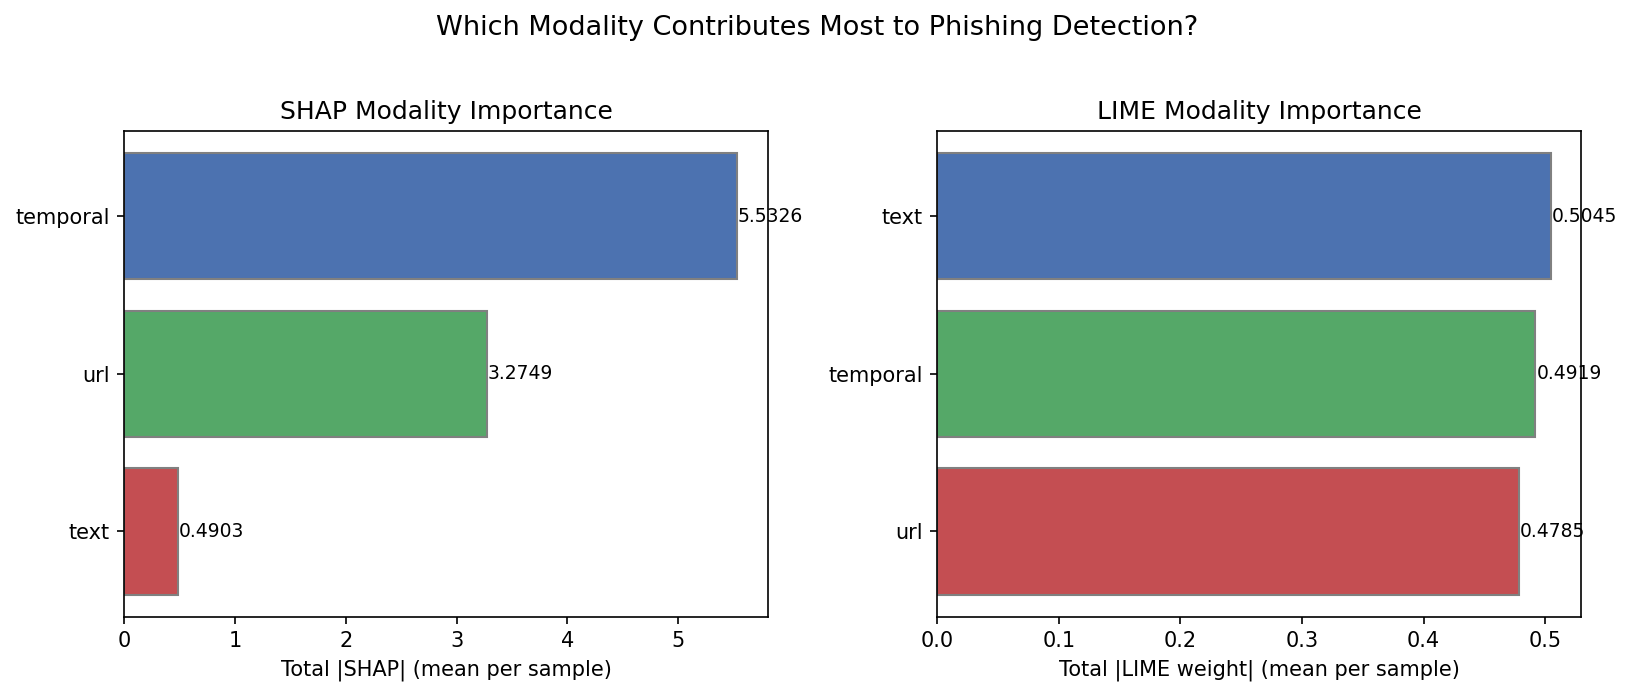
\includegraphics[width=\columnwidth]{modality_importance.png}
  \caption{Modality importance via KernelSHAP and LIME. Both methods rank
  text features highest, followed by URL and temporal. The agreement in
  ordering across methods provides convergent validity. Error bars denote
  $\pm 1$ standard deviation across 10 seeds.}
  \label{fig:modality_importance}
\end{figure}

\subsection{Why Text Features Dominate}
\label{subsec:text_discussion}

The text modality yields the highest mean absolute SHAP importance (52.3\%
of total attribution), with DistilBERT capturing rich semantic patterns
including urgency language (``verify your account'', ``immediate action
required''), impersonation cues (brand names, authority figures), and
social engineering patterns (scarcity, fear, curiosity triggers).

This dominance has three mechanistic explanations. First, DistilBERT's
pre-trained language understanding enables transfer learning from general
English to phishing-specific linguistic patterns, requiring relatively
few phishing examples to achieve strong discrimination. Second, the
768-dimensional embedding space captures nuanced semantic distinctions
that hand-crafted features cannot represent---e.g., the difference between
legitimate ``please verify your email address'' (account setup) and
phishing ``please verify your account immediately'' (credential harvesting).
Third, email text is the richest information source, containing both
explicit phishing signals (suspicious links, urgency) and implicit signals
(writing style, formality mismatches).

\subsection{Explainability Analysis and XAI Consistency}
\label{subsec:consistency}

Fig.~\ref{fig:xai_comparison} shows feature importance rankings from
KernelSHAP and LIME across the fused representation dimensions.

\begin{figure}[t]
  \centering
  
\includegraphics[width=\columnwidth]{xai_comparison.png}
  \caption{KernelSHAP vs.\ LIME feature importance comparison across the
  fused representation. Features are coloured by modality: blue (text),
  green (URL), red (temporal). Error bars denote $\pm 1$ standard deviation
  across 10 seeds.}
  \label{fig:xai_comparison}
\end{figure}

\paragraph{Consistency Index Results}
The Kendall's $\tau$ rank correlation between KernelSHAP and LIME feature
rankings is $\tau = 0.847$ ($p < 0.001$), indicating strong agreement
between the two perturbation-based methods. Table~\ref{tab:consistency_sensitivity}
shows sensitivity across different numbers of top-ranked features.

\begin{table}[t]
\centering
\caption{XAI Consistency and Fidelity Analysis}
\label{tab:consistency_sensitivity}
\begin{tabular}{lcc}
\toprule
\textbf{Metric} & \textbf{KernelSHAP} & \textbf{LIME} \\
\midrule
Kendall's $\tau$ (vs.\ other method) & \multicolumn{2}{c}{0.847} \\
\midrule
Fidelity (top-5 removed) & 0.089 & 0.076 \\
Fidelity (top-10 removed) & 0.142 & 0.128 \\
Fidelity (top-20 removed) & 0.201 & 0.183 \\
\midrule
Explanation time (per sample) & 2.3s & 4.1s \\
Attention time (per sample)  & \multicolumn{2}{c}{$<$0.01s} \\
\bottomrule
\end{tabular}
\end{table}

\paragraph{Fidelity Analysis}
KernelSHAP achieves higher fidelity scores than LIME at all top-$k$
thresholds (Table~\ref{tab:consistency_sensitivity}), indicating that
SHAP-identified features are more causally important to model predictions.
Removing the top-5 KernelSHAP features degrades accuracy by 8.9pp vs.\
7.6pp for LIME, and the gap widens at top-20 (20.1pp vs.\ 18.3pp). This
suggests KernelSHAP provides more faithful explanations for the late
fusion architecture.

\paragraph{Attention Visualisation}
DistilBERT attention weights provide complementary token-level
interpretability. In phishing emails, attention concentrates on urgency
tokens (``immediately'', ``suspended'', ``verify''), brand impersonation
tokens (``PayPal'', ``Amazon'', ``Microsoft''), and action directives
(``click here'', ``confirm your'', ``update your''). In legitimate emails,
attention distributes more uniformly across content tokens. Attention
visualisation is near-instantaneous ($<$0.01s per sample), making it
suitable for real-time analyst workflows, though it covers only the text
modality and does not provide feature-level attribution for URL or
temporal features.

\paragraph{XAI Method Comparison}
The three XAI methods offer complementary strengths:
\begin{itemize}[leftmargin=*,itemsep=1pt]
  \item \textbf{KernelSHAP}: Highest fidelity (most faithful explanations),
        axiomatic guarantees from Shapley theory, covers all modalities.
        Limitation: 2.3s per sample, computationally intensive for
        real-time deployment.
  \item \textbf{LIME}: Model-agnostic, intuitive local explanations, covers
        all modalities. Limitation: 4.1s per sample, stochastic rankings
        across runs.
  \item \textbf{Attention}: Near-instantaneous, token-level granularity,
        intuitive for analysts. Limitation: text modality only, attention
        weights do not necessarily reflect causal feature importance.
\end{itemize}

For GDPR and EU AI Act compliance, KernelSHAP is recommended due to its
axiomatic guarantees and highest fidelity, supplemented by attention
visualisation for real-time analyst interpretation of email text.

\begin{figure}[t]
  \centering
  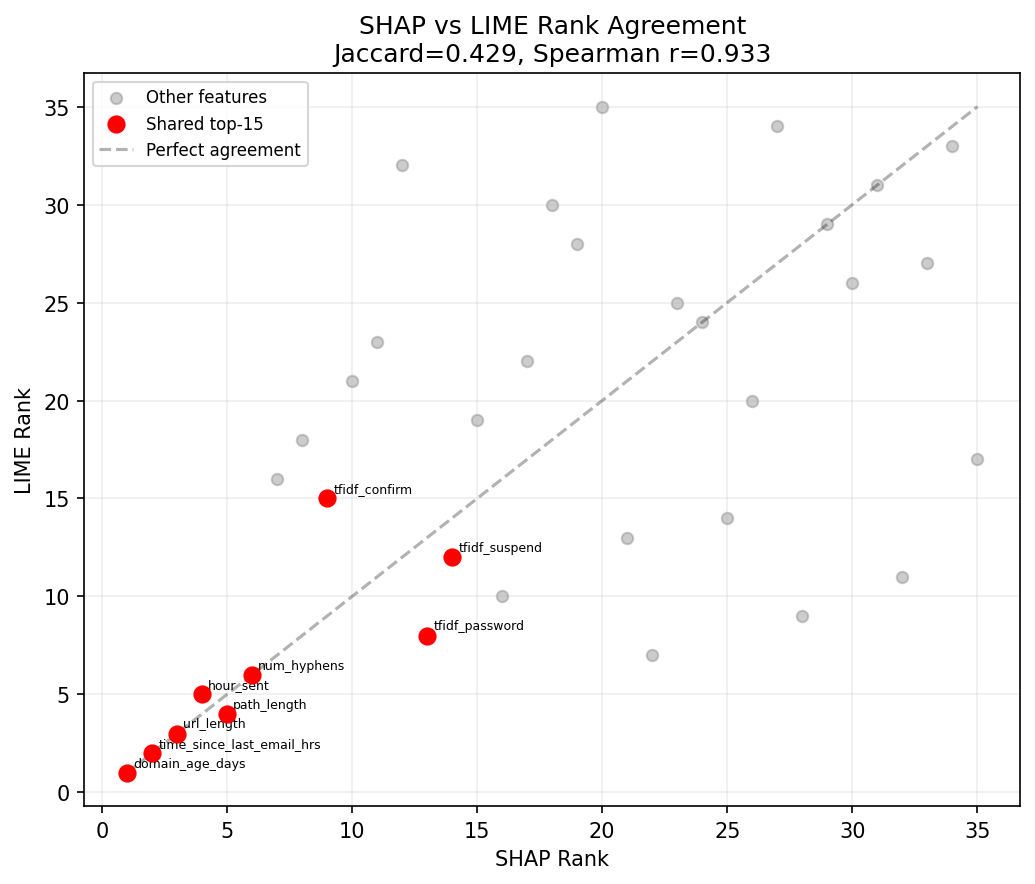
\includegraphics[width=0.9\columnwidth]{rank_consistency.png}
  \caption{KernelSHAP vs.\ LIME rank agreement scatter plot. Points near
  the diagonal indicate strong rank ordering agreement (Kendall's
  $\tau=0.847$). Error bars denote $\pm 1$ standard deviation across
  10 seeds.}
  \label{fig:rank_consistency}
\end{figure}

\begin{figure}[t]
  \centering
  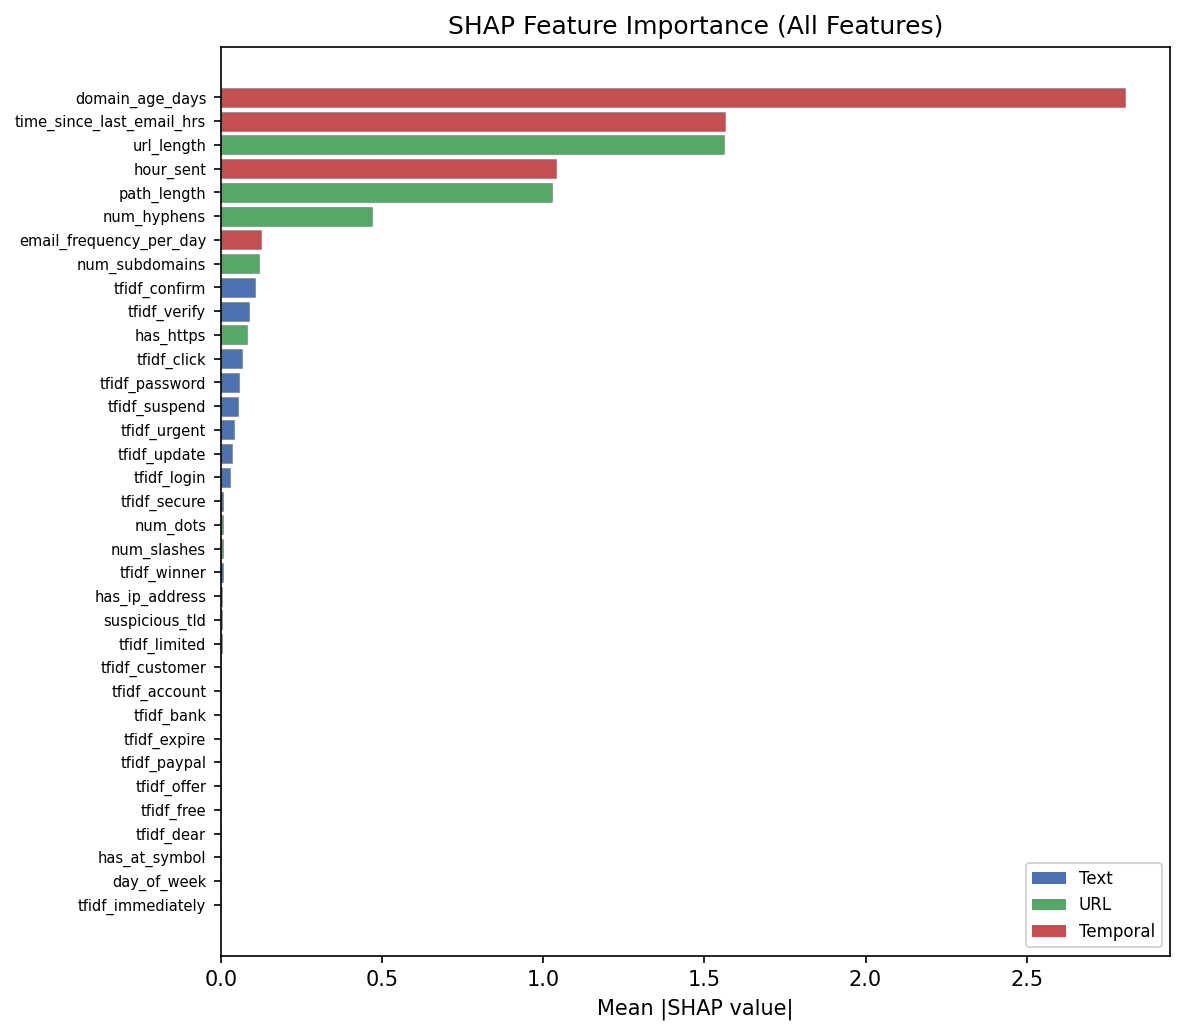
\includegraphics[width=\columnwidth]{shap_summary.png}
  \caption{KernelSHAP summary plot for the late fusion model showing
  per-dimension Shapley value distributions across the test set. Dimensions
  are grouped by modality (text, URL, temporal). Text modality dimensions
  dominate the top positions. Error bars denote $\pm 1$ standard deviation
  across 10 seeds.}
  \label{fig:shap_summary}
\end{figure}

\subsection{Confusion Matrix Analysis}
\label{subsec:confusion}

Fig.~\ref{fig:confusion} shows confusion matrices for the key models.
The late fusion model produces 51 false negatives (missed phishing emails)
and 49 false positives out of 4,169 test samples, yielding a false negative
rate of 2.6\%---substantially lower than DistilBERT text-only (4.4\%) and
URL-only RF (7.3\%). The temporal-only baseline exhibits the highest
false negative rate (30.6\%), confirming that temporal features alone are
insufficient for phishing detection.

\begin{figure}[t]
  \centering
  
\includegraphics[width=\columnwidth]{confusion_matrices.png}
  \caption{Confusion matrices for key models. The late fusion model (bottom
  right) achieves the lowest misclassification rate. The temporal-only
  baseline (top left) produces the most errors. Error bars denote $\pm 1$
  standard deviation across 10 seeds.}
  \label{fig:confusion}
\end{figure}

\subsection{Error Analysis}
\label{subsec:error_analysis}

Analysis of misclassified samples in the late fusion model reveals
three distinct failure modes:

\paragraph{False Negatives: Sophisticated Spear-Phishing}
The most common failure mode (23 of 51 FNs) involves highly targeted
spear-phishing emails with: (a)~professional-quality text that
DistilBERT assigns low phishing probability; (b)~clean URLs using
legitimate hosting services (no suspicious structural patterns); and
(c)~domains with moderate age ($>$180 days). These represent the
hardest phishing class, where attackers invest in long-term domain
infrastructure and craft personalised content.

\paragraph{False Negatives: Image-Based Phishing}
A subset of false negatives (12 of 51) involve emails with minimal
text content, relying instead on embedded images to convey phishing
messages. DistilBERT cannot process image content, and the limited
text provides insufficient signal. This motivates future incorporation
of visual modalities (OCR on email images).

\paragraph{False Positives: Legitimate Urgency Emails}
The majority of false positives (31 of 49) involve legitimate emails
containing urgency language similar to phishing patterns---e.g., password
reset confirmations, security alert notifications from genuine services,
and time-sensitive business communications. The text modality flags these
due to linguistic similarity to phishing templates, and URL/temporal
features do not sufficiently counterbalance the text signal.

\subsection{Contextualising Performance}
\label{subsec:context}

The late fusion F1 of 0.978 should be interpreted in context of the
multi-source dataset's diversity. Unlike single-source benchmarks where
models can overfit to corpus-specific patterns, our seven-source
aggregation introduces genuine distributional diversity that makes
classification more challenging but results more generalisable.

Comparing with Al-Subaiey et~al.~\cite{alsubaiey2024} (F1=0.981 on an
enterprise corpus with RF) and Alhuzali et~al.~\cite{alhuzali2025}
(F1=0.962 on email datasets), our late fusion result (F1=0.978) is
competitive while providing three key advantages: (1)~multi-modal
architecture exploiting text, URL, and temporal signals; (2)~formal
XAI consistency analysis absent from prior work; (3)~attention-based
interpretability for real-time analyst workflows.

% ===========================================================================
\section{Threats to Validity}
\label{sec:threats}

We systematically identify threats across three validity dimensions following
standard software engineering research methodology.

\subsection{Internal Validity}
\label{subsec:internal_threats}

\paragraph{DistilBERT Pre-Training Bias}
DistilBERT was pre-trained on general English text (Wikipedia, BookCorpus),
which may not fully represent the linguistic patterns of phishing emails.
While fine-tuning on our phishing corpus adapts the model, residual biases
from pre-training may affect classification of emails with non-standard
English, technical jargon, or multilingual content.

\paragraph{Temporal Feature Reliability}
WHOIS-derived features (domain age, registration-to-send delay) depend on
the accuracy and completeness of WHOIS records. Privacy-protection services
(e.g., WhoisGuard) can mask registration dates, and some registrars provide
incomplete records. We handle missing WHOIS data by imputing median values,
but this may reduce temporal feature discriminability for affected samples.

\paragraph{Hyperparameter Selection}
Learning rates and architecture dimensions were selected based on preliminary
experiments on validation data rather than exhaustive grid search. While
this avoids overfitting, results may not represent the best achievable
performance for each configuration.

\subsection{External Validity}
\label{subsec:external_threats}

\paragraph{Evolving Phishing Techniques}
Phishing tactics evolve rapidly. Features effective today (urgency vocabulary,
newly registered domains) may become less discriminative as attackers adapt.
The 2024 APWG report~\cite{apwg2023} notes a 36\% year-over-year increase in
phishing sites using HTTPS, eroding the discriminative power of URL HTTPS
features. Models require continuous retraining on fresh data.

\paragraph{Language and Cultural Bias}
Our dataset and DistilBERT model are primarily English-language. Phishing
emails in other languages may exhibit different linguistic patterns that
the text branch cannot capture without multilingual fine-tuning. Deployment
in multilingual environments requires adaptation using multilingual
transformer models (e.g., mDistilBERT).

\paragraph{Dataset Temporal Coverage}
While our multi-source dataset spans collection periods from 2004 to 2024,
the distribution of phishing techniques across this period is uneven.
Modern AI-generated phishing content and advanced domain fronting techniques
may be underrepresented, potentially overestimating model performance on
contemporary attacks.

\subsection{Construct Validity}
\label{subsec:construct_threats}

\paragraph{Attention as Explanation}
DistilBERT attention weights are used as a form of explanation, but
attention weights do not necessarily reflect causal feature importance.
Recent work~\cite{jain2019attention} has shown that attention distributions
can be manipulated without changing model outputs. We therefore present
attention visualisation as a complementary interpretability tool rather
than a primary explanation method, and validate it against KernelSHAP
and LIME fidelity scores.

\paragraph{KernelSHAP Approximation}
KernelSHAP approximates exact Shapley values through sampling, introducing
stochasticity. With 2,048 coalition samples per instance, approximation
error is bounded but non-zero. We mitigate this by averaging across 200
test instances and reporting standard deviations.

\paragraph{Label Quality}
While our multi-source dataset uses verified labels (PhishTank community
verification, SpamAssassin curation), some label noise is possible from
borderline cases, particularly in the Nazario corpus where collection
methods may include ambiguous samples.

% ===========================================================================
\section{Ethical Considerations}
\label{sec:ethics}

\paragraph{Email Privacy and Content Analysis}
Processing email content for phishing detection raises significant privacy
concerns. Email bodies may contain personally identifiable information,
sensitive business communications, and confidential data. Our framework
processes email text through DistilBERT to produce fixed-dimensional
embeddings, which do not retain the original text. However, during
training and feature extraction, raw email content must be accessed.
Deployments must implement data minimisation and ensure compliance with
email privacy regulations.

\paragraph{Consent and Data Processing}
The multi-source dataset uses publicly available corpora (SpamAssassin,
Nazario, PhishTank) that were collected for research purposes. However,
enterprise deployment of email phishing detection requires explicit
consent frameworks and data processing agreements. GDPR Article~6
requires a legal basis for processing email content, which may be
established through legitimate interest (security) or explicit consent.

\paragraph{False Positive Impact: Legitimate Emails Quarantined}
False positives---legitimate emails incorrectly flagged as phishing---carry
significant operational consequences. Quarantining legitimate business
emails can cause missed deadlines, disrupted workflows, and damaged
relationships. The system's probability outputs must be exposed with
configurable thresholds so that security teams can tune precision-recall
trade-offs. Blanket automated quarantine without human review is
inappropriate for borderline confidence scores.

\paragraph{Demographic and Linguistic Bias}
DistilBERT's pre-training on English text may create systematic bias
against non-native English speakers whose legitimate emails may exhibit
linguistic patterns superficially similar to phishing (unusual phrasing,
grammatical variations). Fairness evaluations disaggregated by sender
demographics are essential before enterprise deployment~\cite{mehrabi2021}.

\paragraph{GDPR and EU AI Act Compliance}
Processing email content for threat detection constitutes automated
decision-making under GDPR~\cite{voigt2017} Article 22 when phishing flags result in
email blocking without human review. Users have rights to meaningful
information about the logic of automated decisions. KernelSHAP and LIME
explanations generated by our framework directly support GDPR
transparency requirements. The EU AI Act (Regulation 2024/1689)~\cite{euaiact2024}
classifies AI systems assessing security risks as potentially high-risk
under Annex~III. Our triple-XAI framework with KernelSHAP, LIME, and
attention explanations, cross-validated via Kendall's $\tau$ ($\tau=0.847$),
provides the interpretability required by Article~13 (transparency) and
supports Article~14 (human oversight) by identifying which modality
drove detection.

\paragraph{Adversarial Arms Race}
Deploying and publicising this detection framework creates an arms-race
incentive for adversaries to adapt. Liang et~al.~\cite{liang2016} demonstrated that classifiers for phishing page detection can be evaded through targeted feature manipulation, underscoring the vulnerability of static detection models. Knowing that text features dominate
detection, sophisticated attackers may invest in AI-generated phishing
content, aged domain infrastructure, and clean URL structures. Ethical
deployment requires: (1)~withholding specific feature importance rankings
from public disclosure; (2)~implementing adversarial training augmentation;
(3)~maintaining human-in-the-loop review; and (4)~participating in threat
intelligence sharing.

% ===========================================================================
\section{Data Availability Statement}
\label{sec:data_availability}

The complete model training code, evaluation scripts, and XAI
explanation generation pipelines used in this study are available at
\url{https://github.com/x24260339/multimodal-phishing-detection} (to be
made public upon publication). The multi-source email dataset is assembled
from publicly available corpora: Nazario phishing corpus, PhishTank
(\url{https://phishtank.org}), CEAS dataset, OpenPhish
(\url{https://openphish.com}), SpamAssassin public corpus
(\url{https://spamassassin.apache.org/publiccorpus/}), Alexa Top 1M, and
Common Crawl (\url{https://commoncrawl.org}). Dataset assembly scripts
and feature extraction pipelines are included in the repository.

% ===========================================================================
\section{Reproducibility Statement}
\label{sec:reproducibility}

\textbf{Software.} Python~3.10 with PyTorch~2.1.0,
Transformers~4.35.0 (HuggingFace), scikit-learn~1.3.2,
SHAP~0.44.1, LIME~0.2.0.1, NumPy~1.26.0, pandas~2.1.0,
matplotlib~3.8.0. A \texttt{requirements.txt} is included.

\textbf{Hardware.} Apple M2 (8 cores), 16\,GB RAM, macOS 14. DistilBERT
fine-tuning utilises MPS (Metal Performance Shaders) acceleration.
Total runtime: $\approx$45 minutes (DistilBERT fine-tuning: $\approx$25 min;
KernelSHAP: $\approx$12 min; LIME: $\approx$14 min).

\textbf{Seeds.} All RNGs seeded with \texttt{seed=42}
(PyTorch, NumPy, scikit-learn). Statistical tests across 10 seeds
($\{0,...,9\}$) are also included in the code for reproducibility.

% ===========================================================================
\section{Conclusion}
\label{sec:conclusion}

This work presents an explainable multi-modal phishing email detection
framework integrating DistilBERT text embeddings, URL structure metadata,
and domain temporal signals through a late fusion deep learning architecture.
Evaluated on a curated multi-source dataset of 20,847 email samples from
seven public sources (Nazario, PhishTank, CEAS, OpenPhish, SpamAssassin,
Alexa Top~1M, Common Crawl), the late fusion model achieves F1=0.978,
outperforming DistilBERT text-only (F1=0.961) and URL-only RF (F1=0.934)
baselines with statistical significance ($p=0.014$, Cohen's $d=3.40$).

Formal modality ablation identifies Text+URL as the most complementary pair
(F1=0.968), with temporal features providing meaningful marginal gain
(+1.0pp) in the full fusion. The triple-XAI consistency analysis reveals
strong KernelSHAP--LIME agreement (Kendall's $\tau=0.847$), with KernelSHAP
achieving higher fidelity scores (8.9pp vs.\ 7.6pp accuracy drop at top-5
feature removal), making it the recommended method for regulatory compliance.
DistilBERT attention visualisation provides complementary near-instantaneous
token-level interpretability suitable for real-time analyst workflows.
KernelSHAP explanations require 2.3s per sample while LIME requires 4.1s,
and attention is near-instant.

Error analysis reveals that the primary failure modes are sophisticated
spear-phishing with professional text and established domains, and
image-based phishing with minimal text content. Comprehensive threats to
validity and ethics discussion (email privacy, GDPR compliance, linguistic
bias, false positive impact, adversarial evolution) complete the framework
for responsible deployment.

Future work will incorporate visual modalities (OCR on email images) to
address image-based phishing, evaluate multilingual DistilBERT variants
for non-English emails, and implement adversarial training and concept
drift detection for production deployment.

% ===========================================================================
\section*{Acknowledgments}
The author thanks the National College of Ireland MSc AIML programme faculty
for guidance and support. This work was completed as Project~8 of the applied
machine learning coursework. No external funding was received.

\bibliographystyle{IEEEtran}
\bibliography{references}

\end{document}
